\documentclass[notheorems,table]{beamer}
\usepackage{mybeamer}

%% now the PRESENTATION Starts!
\begin{document}
\graphicspath{{figs/}}

\title{Compressed Sensing for Energy--Efficient Wireless Telemonitoring}
\subtitle{Challenges and Opportunities}
\author[zhilinzhang@ieee.org]{Zhilin Zhang$^1$, Bhaskar D. Rao$^2$, Tzyy-Ping Jung$^3$}
\institute{$^1$ Samsung R\&D Institute America, $^2$ ECE Dept, UCSD, $^3$ Swartz Center for Computational Neuroscience, UCSD}
\date{\bf Asilomar, \today}
\subject{Asilomar 2013}

% Delete this, if you do not want the table of contents to pop up at
% the beginning of each subsection:
%\AtBeginSubsection[]
%{
%  \begin{frame}<beamer>{Outline}
%    \tableofcontents[currentsection,currentsubsection]
%  \end{frame}
%}
%\AtBeginSection[]
%{
%  \begin{frame}<beamer>{Topics(\magt{\sc Next.})}
%    \tableofcontents[currentsection,currentsubsection]
%  \end{frame}
%}

%%------------------------------------------------------------------------%%
% make Opening
\begin{frame}
	\titlepage
\end{frame}

% TOC
%\begin{frame}{Contents}
%	\tableofcontents
%\end{frame}

% - Exactly two or three sections (other than the summary).
% - At *most* three subsections per section.
% - Talk about 30s to 2min per frame. So there should be between about
%   15 and 30 frames, all told.

%%------------------------------------------------------------------------%%
\begin{frame}{Introduction: Low Energy Compression via CS}
% you must skip one line below the frame
    
    {\centering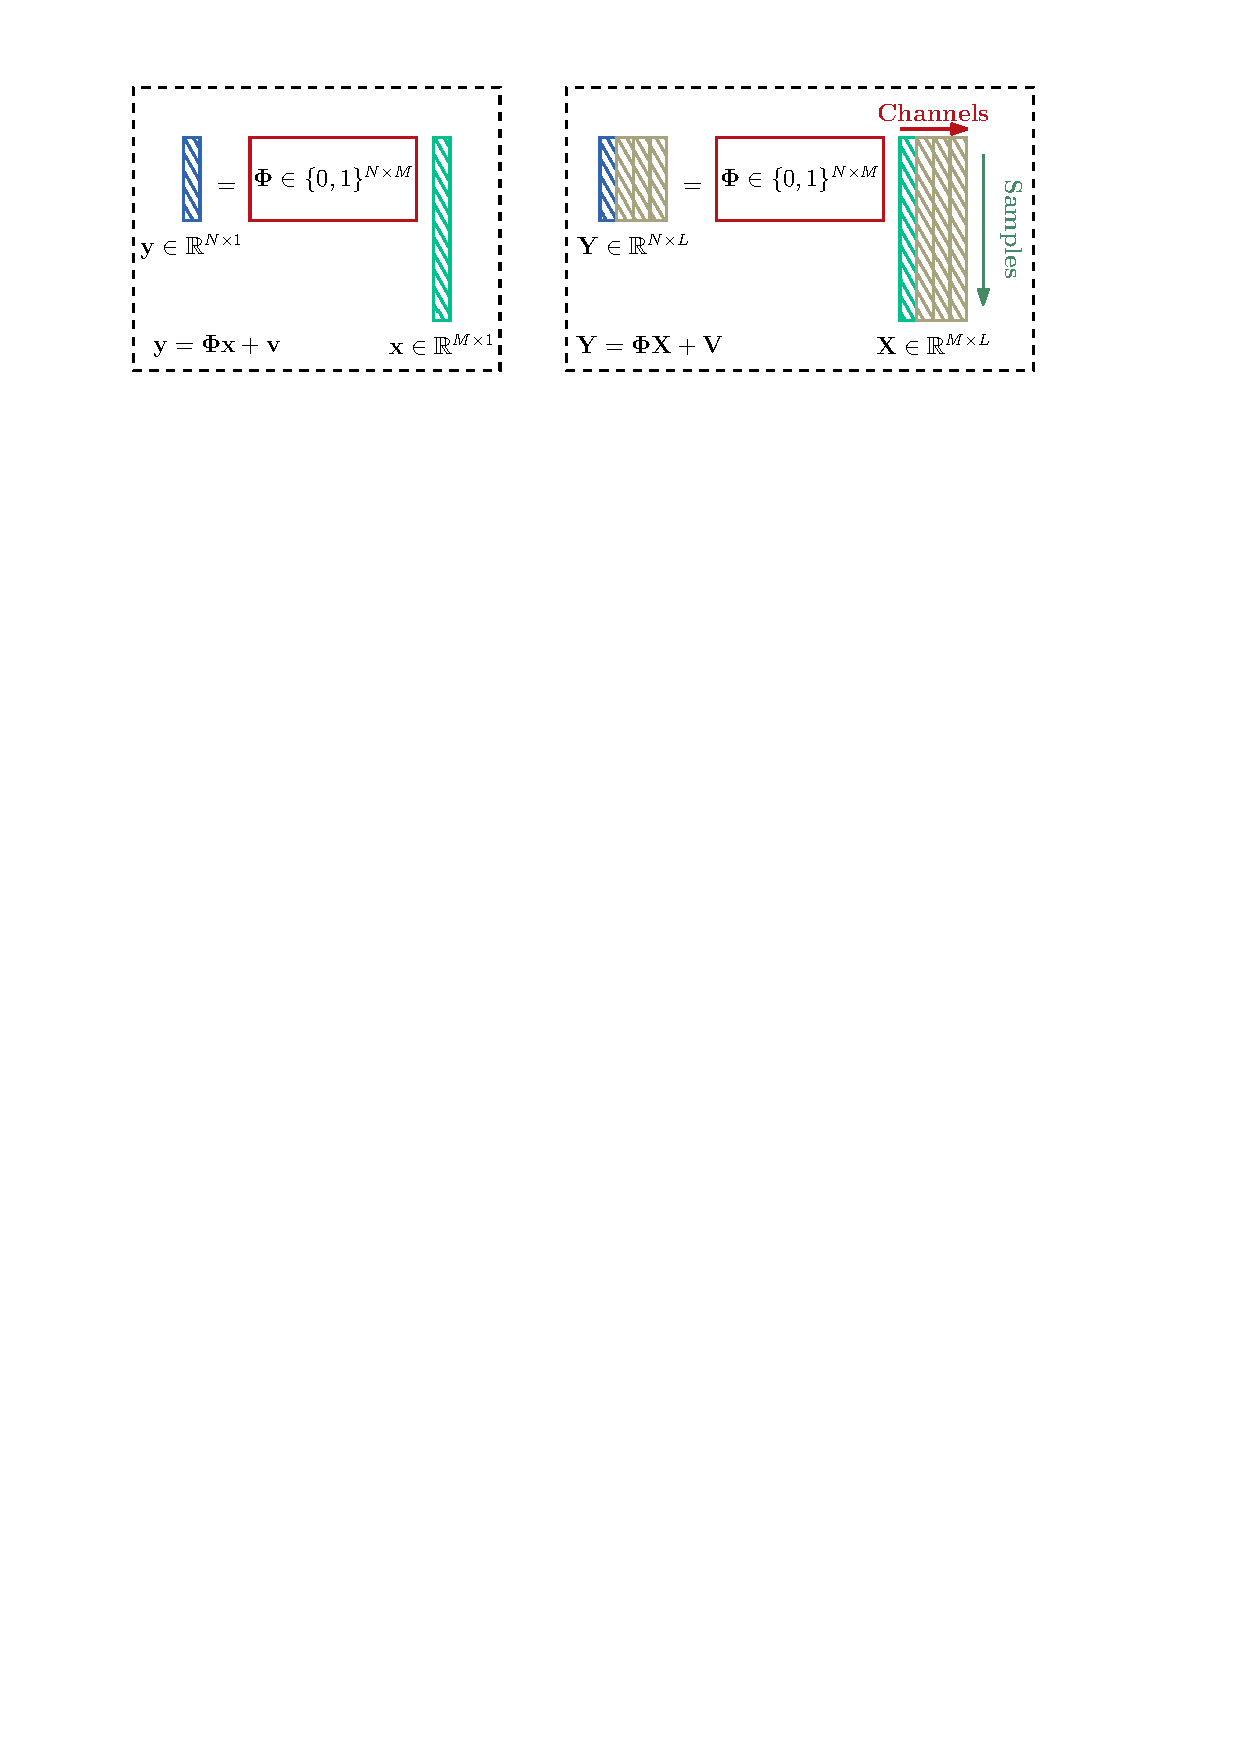
\includegraphics[width=\linewidth]{compress_via_cs.pdf}}
    \begin{itemize}
        \item[1] Consumes much less energy
        \item[2] Recover in the transformed domain where $\ve{y}=(\bm{\Phi}\ve{D})\ve{z}$ and $\ve{x}=\ve{D}\ve{z}$
        \item[3] Multi-channel Biosignals : MMV Model
    \end{itemize}
\end{frame}

%%------------------------------------------------------------------------%%
\begin{frame}{The Challenge : Non-Sparsity}
    
    \magt{insert Fig 3 a, b, c, d here}
    {\centering%
        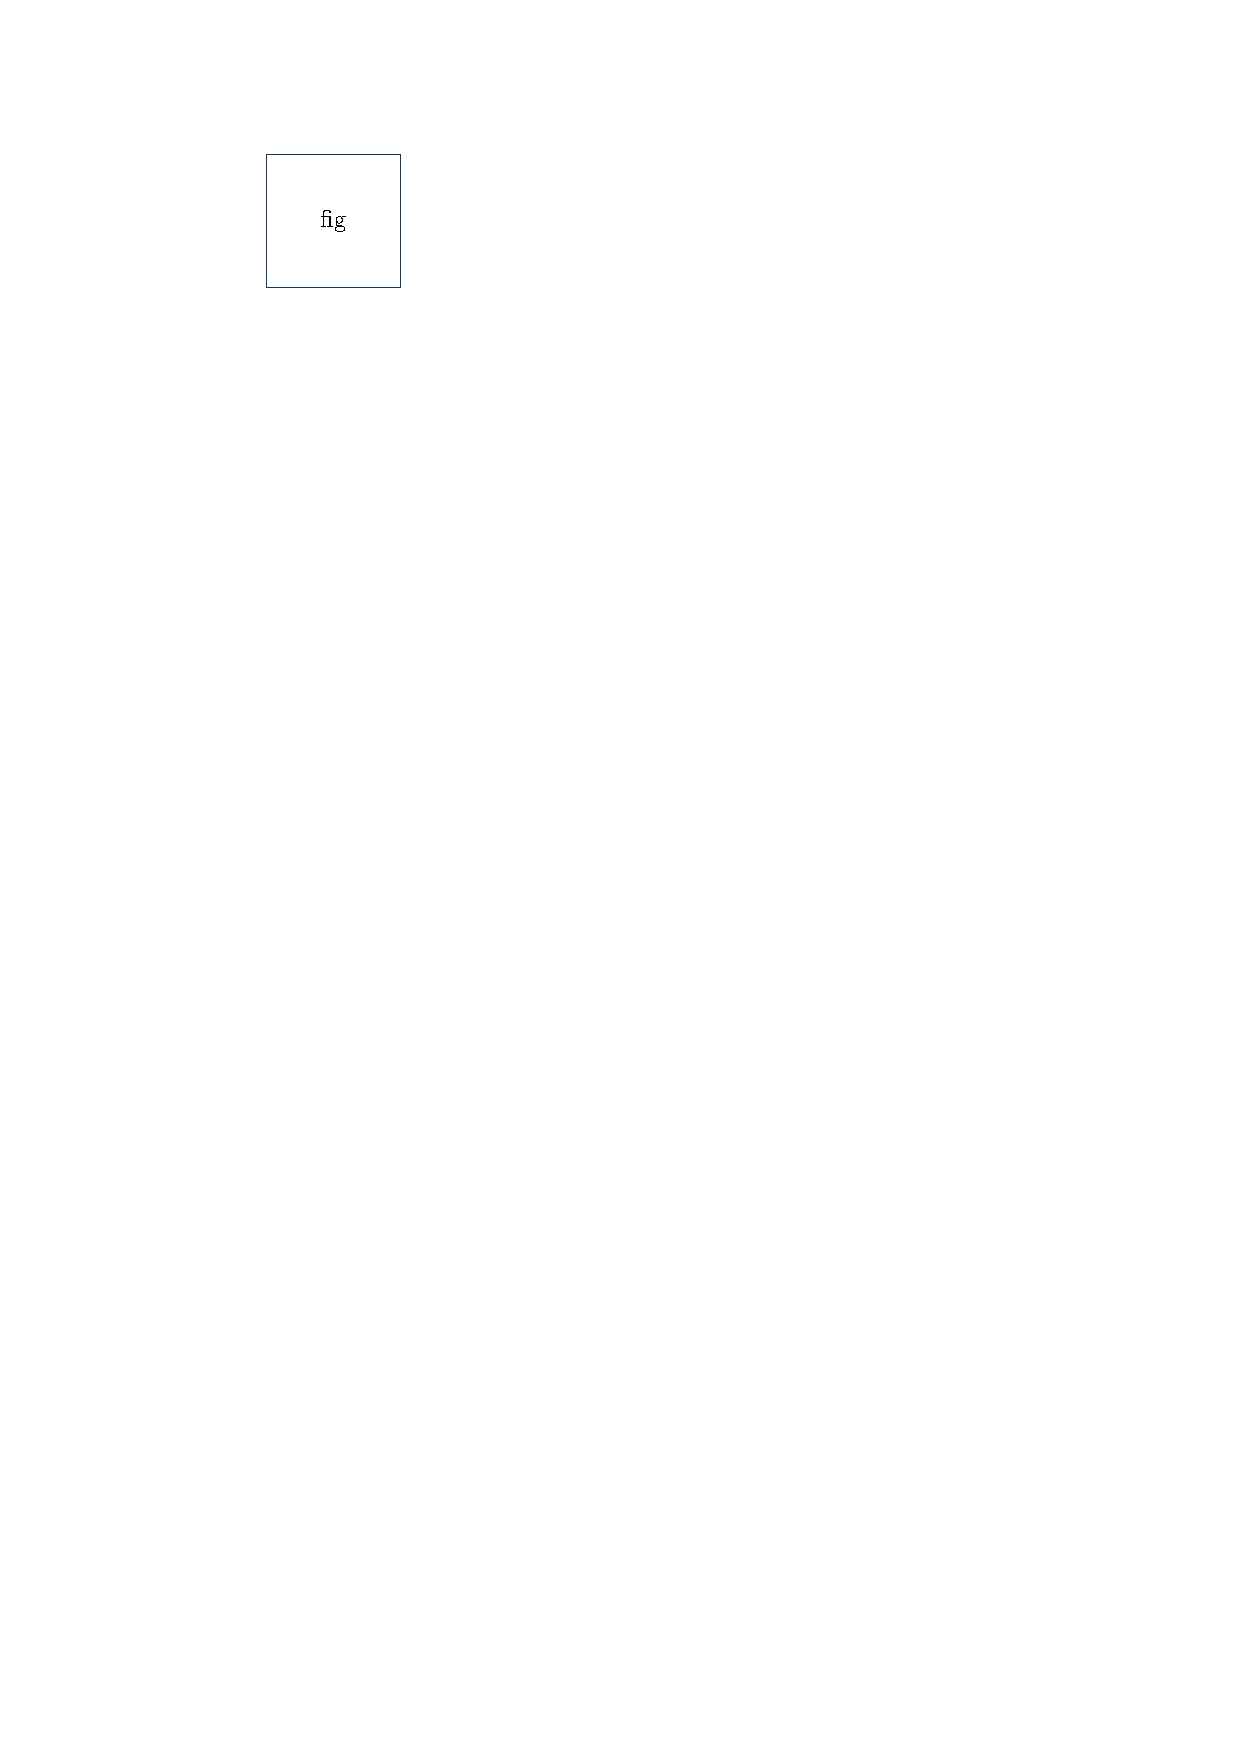
\includegraphics[width=.24\linewidth]{null}~
        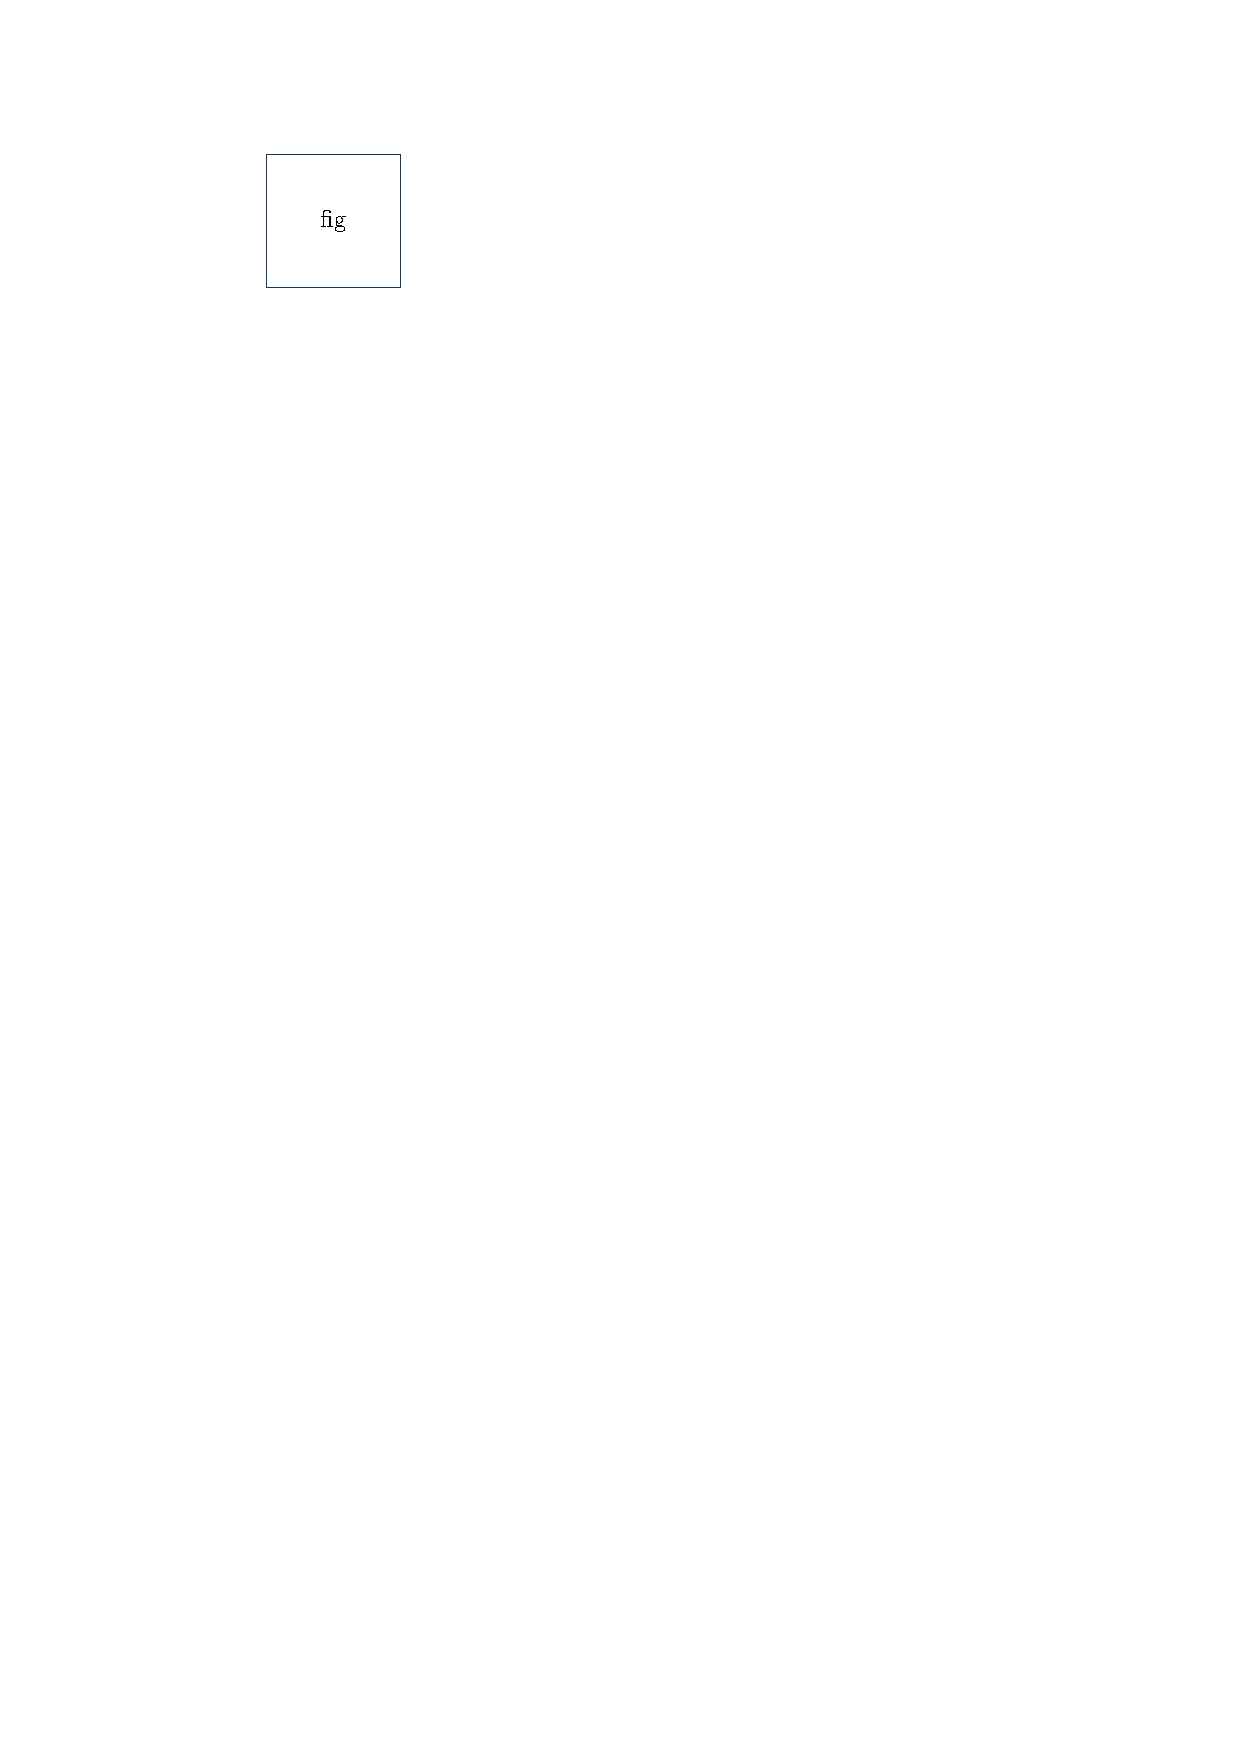
\includegraphics[width=.24\linewidth]{null}~
        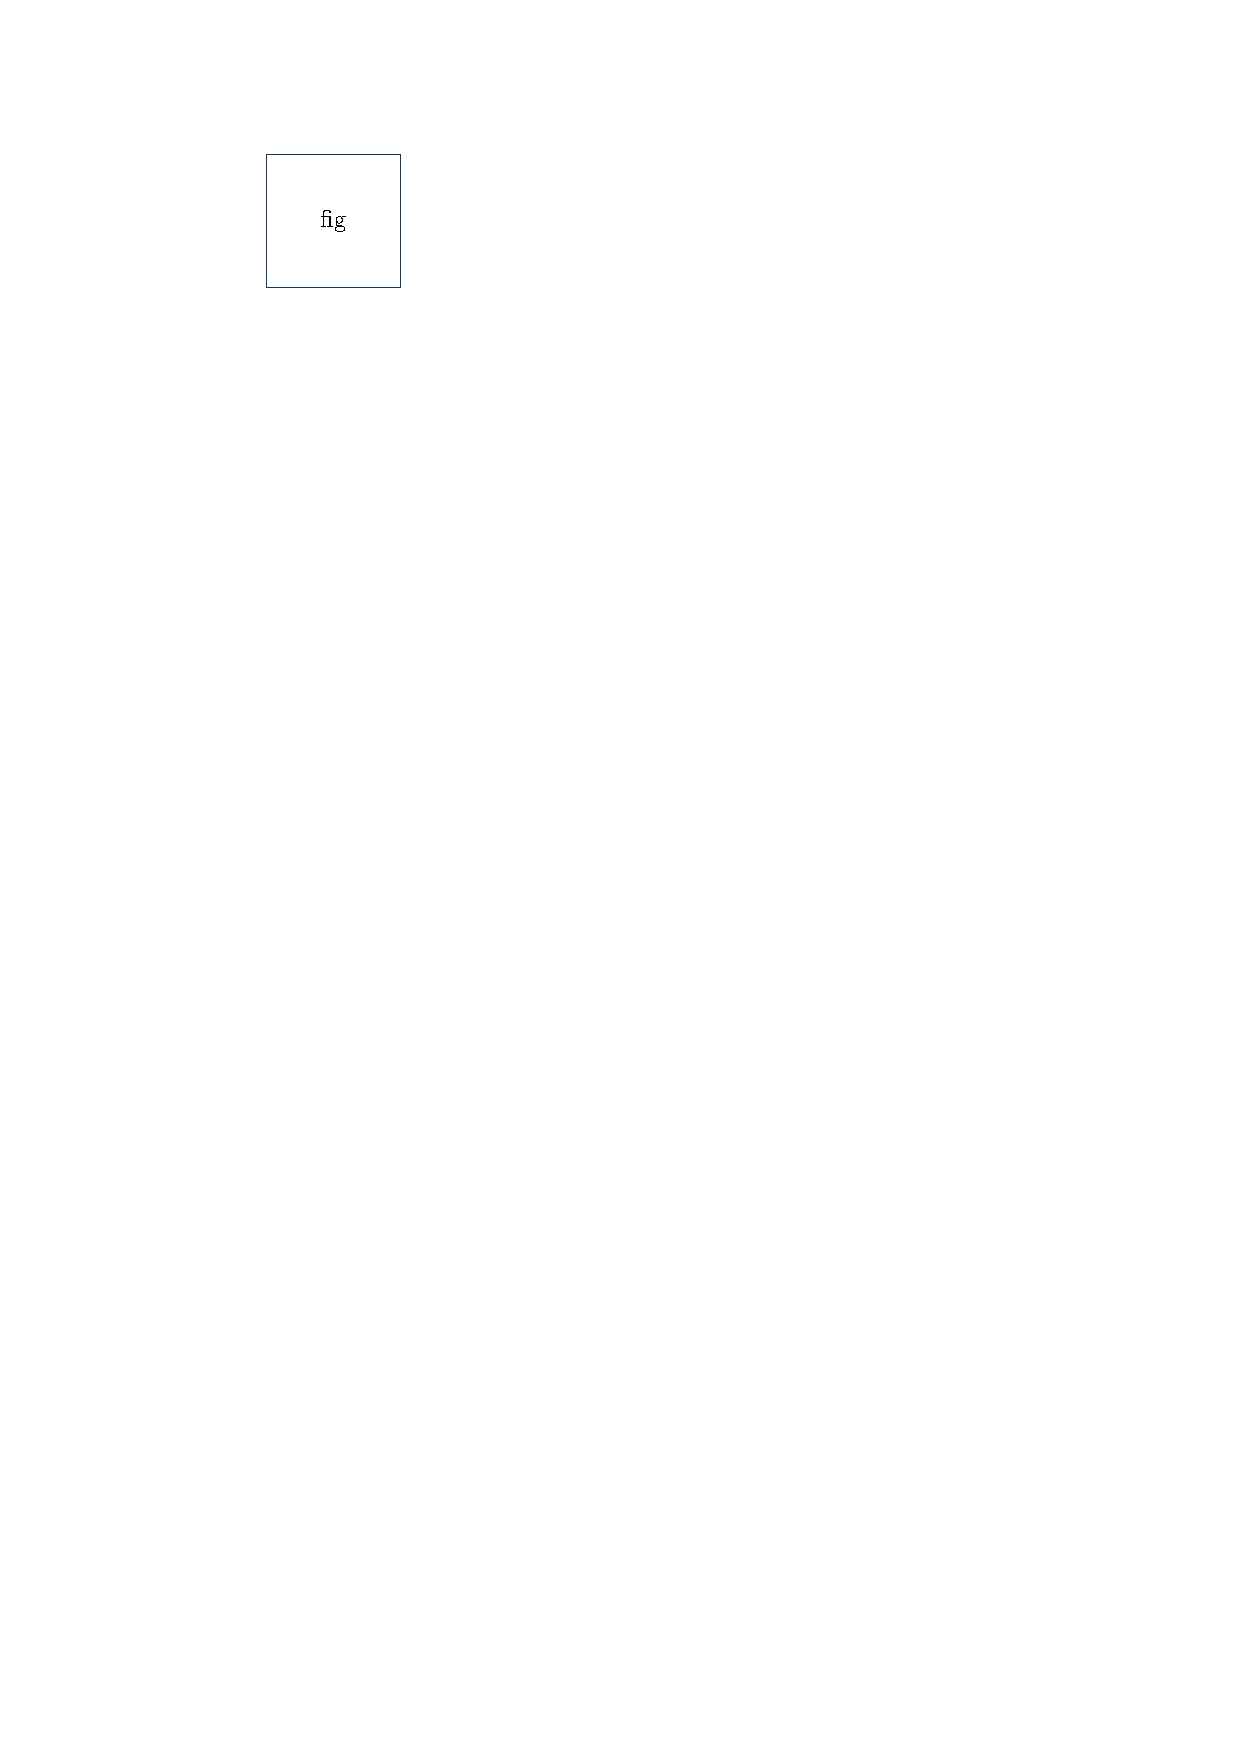
\includegraphics[width=.24\linewidth]{null}~
        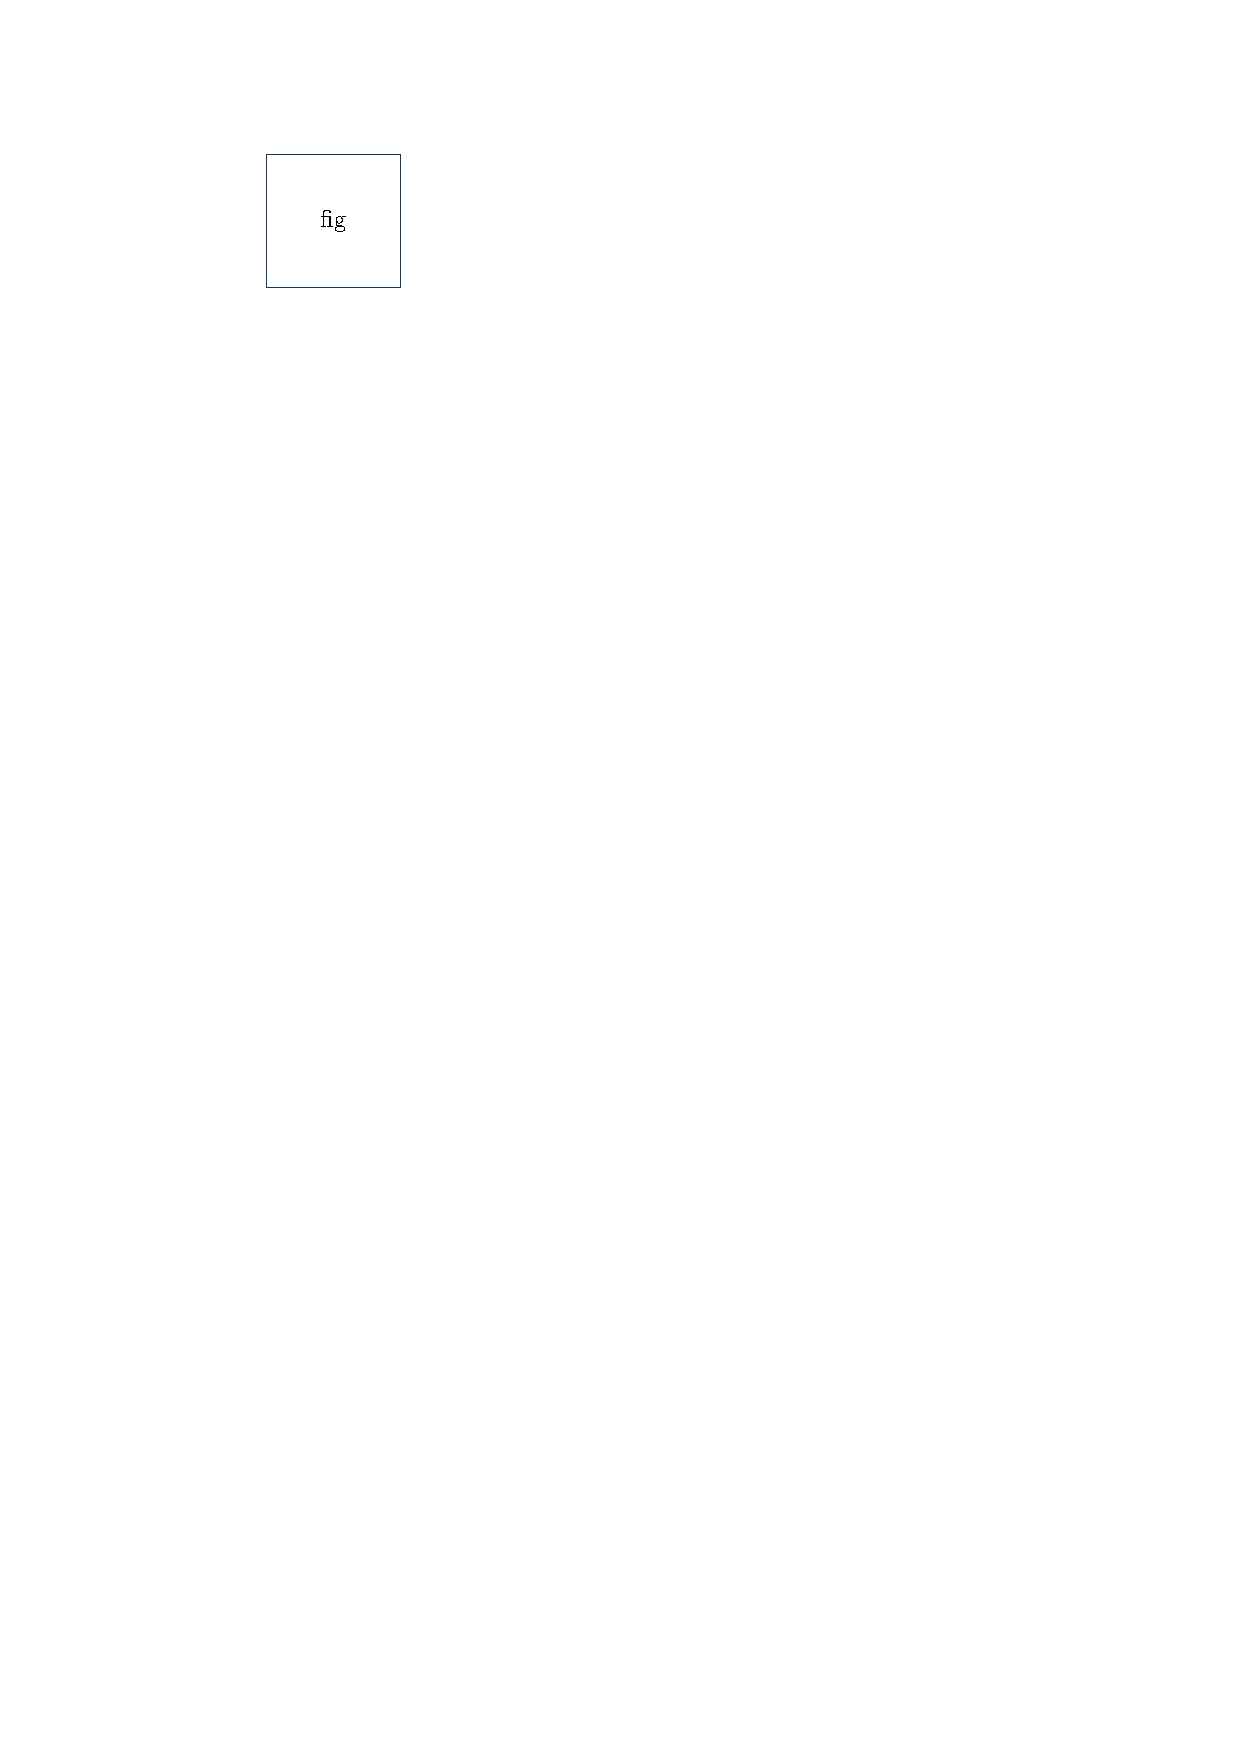
\includegraphics[width=.24\linewidth]{null}~
    }

    \begin{minipage}{.25\linewidth}
        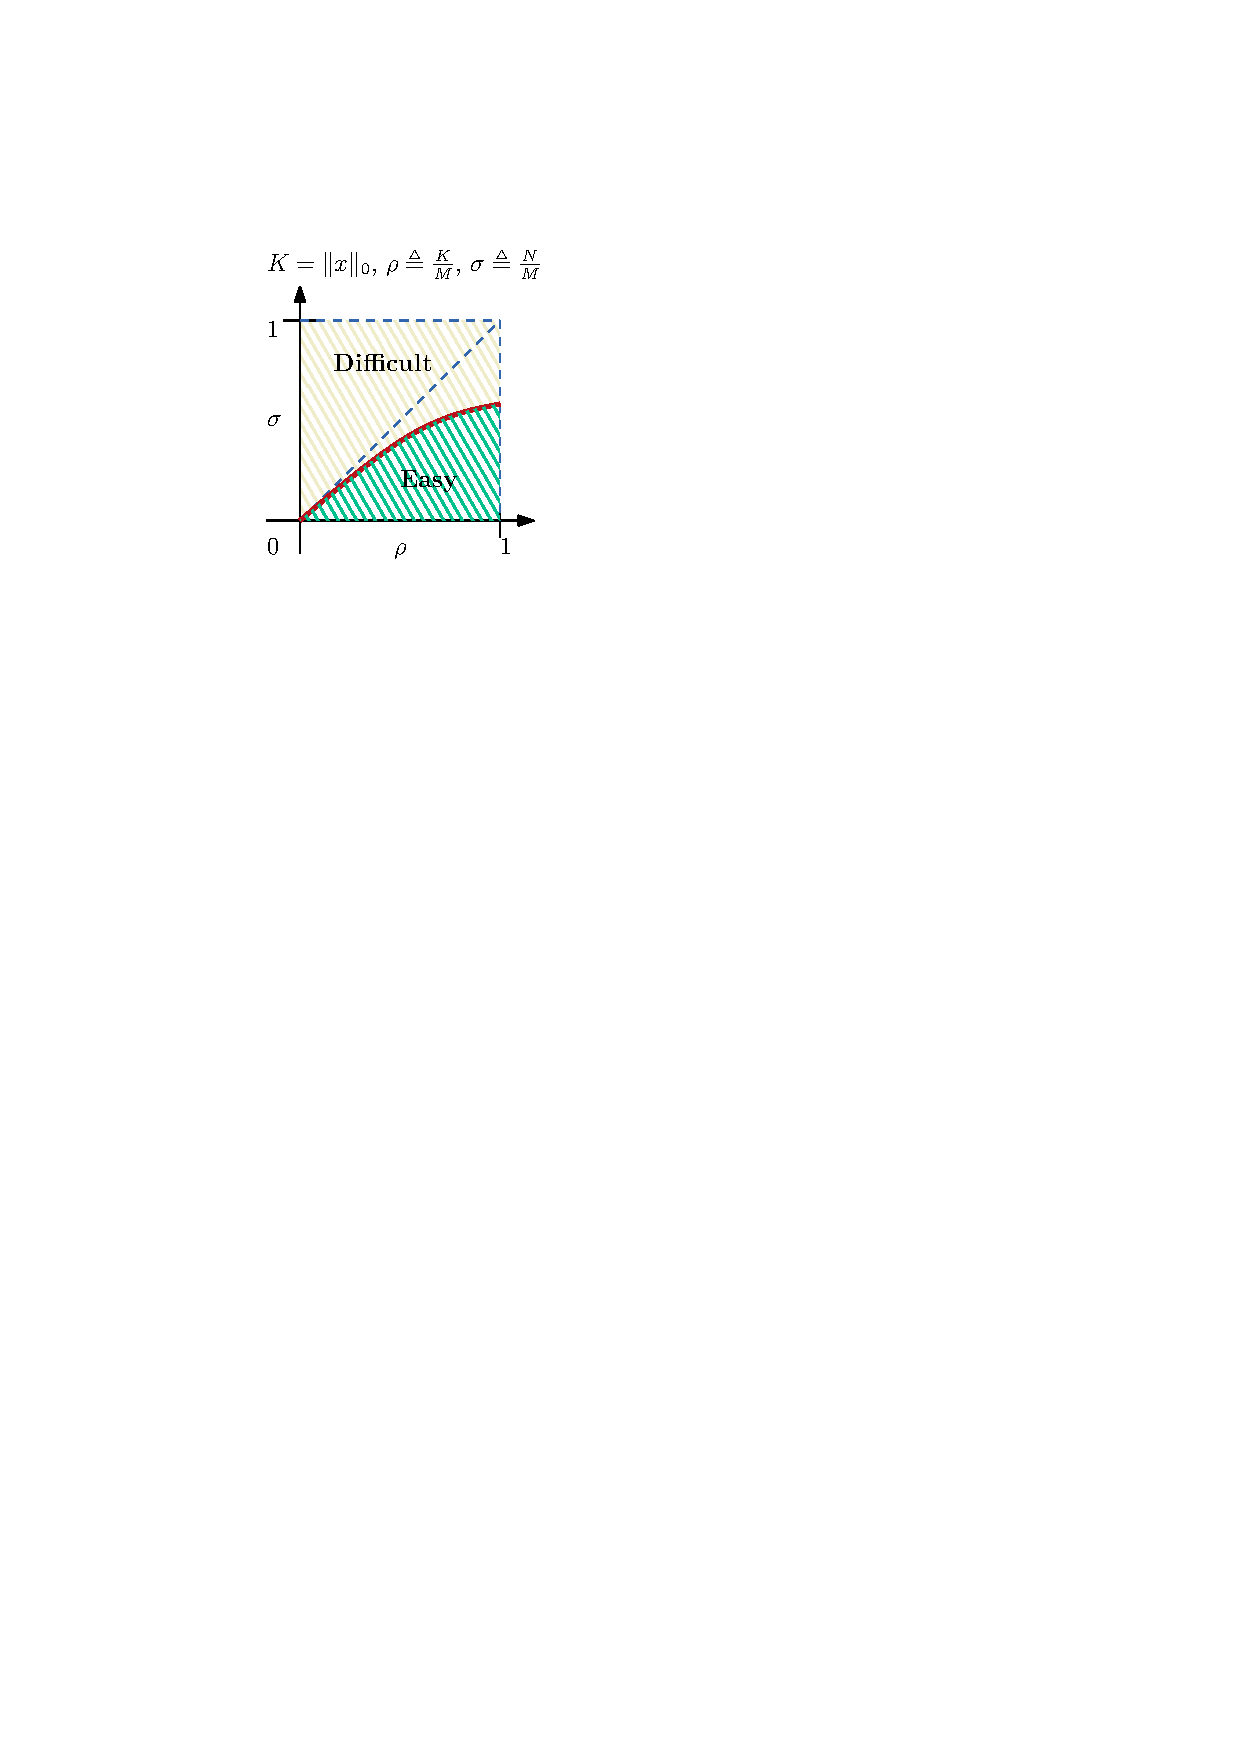
\includegraphics[width=\linewidth]{phase_transition_illustrate.pdf}
    \end{minipage}
    \begin{minipage}{.74\linewidth}
        \begin{itemize}
            \item[1] Biosignals are non-sparse in time or some transformed domains,
            \item[2] Non-sparsity comes from artefacts or low sampling rate,
            \item[3] Artefact removal raises cost in hardware and energy consumptions,
            \item[4] Non-sparse poses challenges for fidelity recovery,
        \end{itemize}
    \end{minipage}
\end{frame}

%%------------------------------------------------------------------------%%
\begin{frame}{State-of-the-art : BSBL-BO}

    {\centering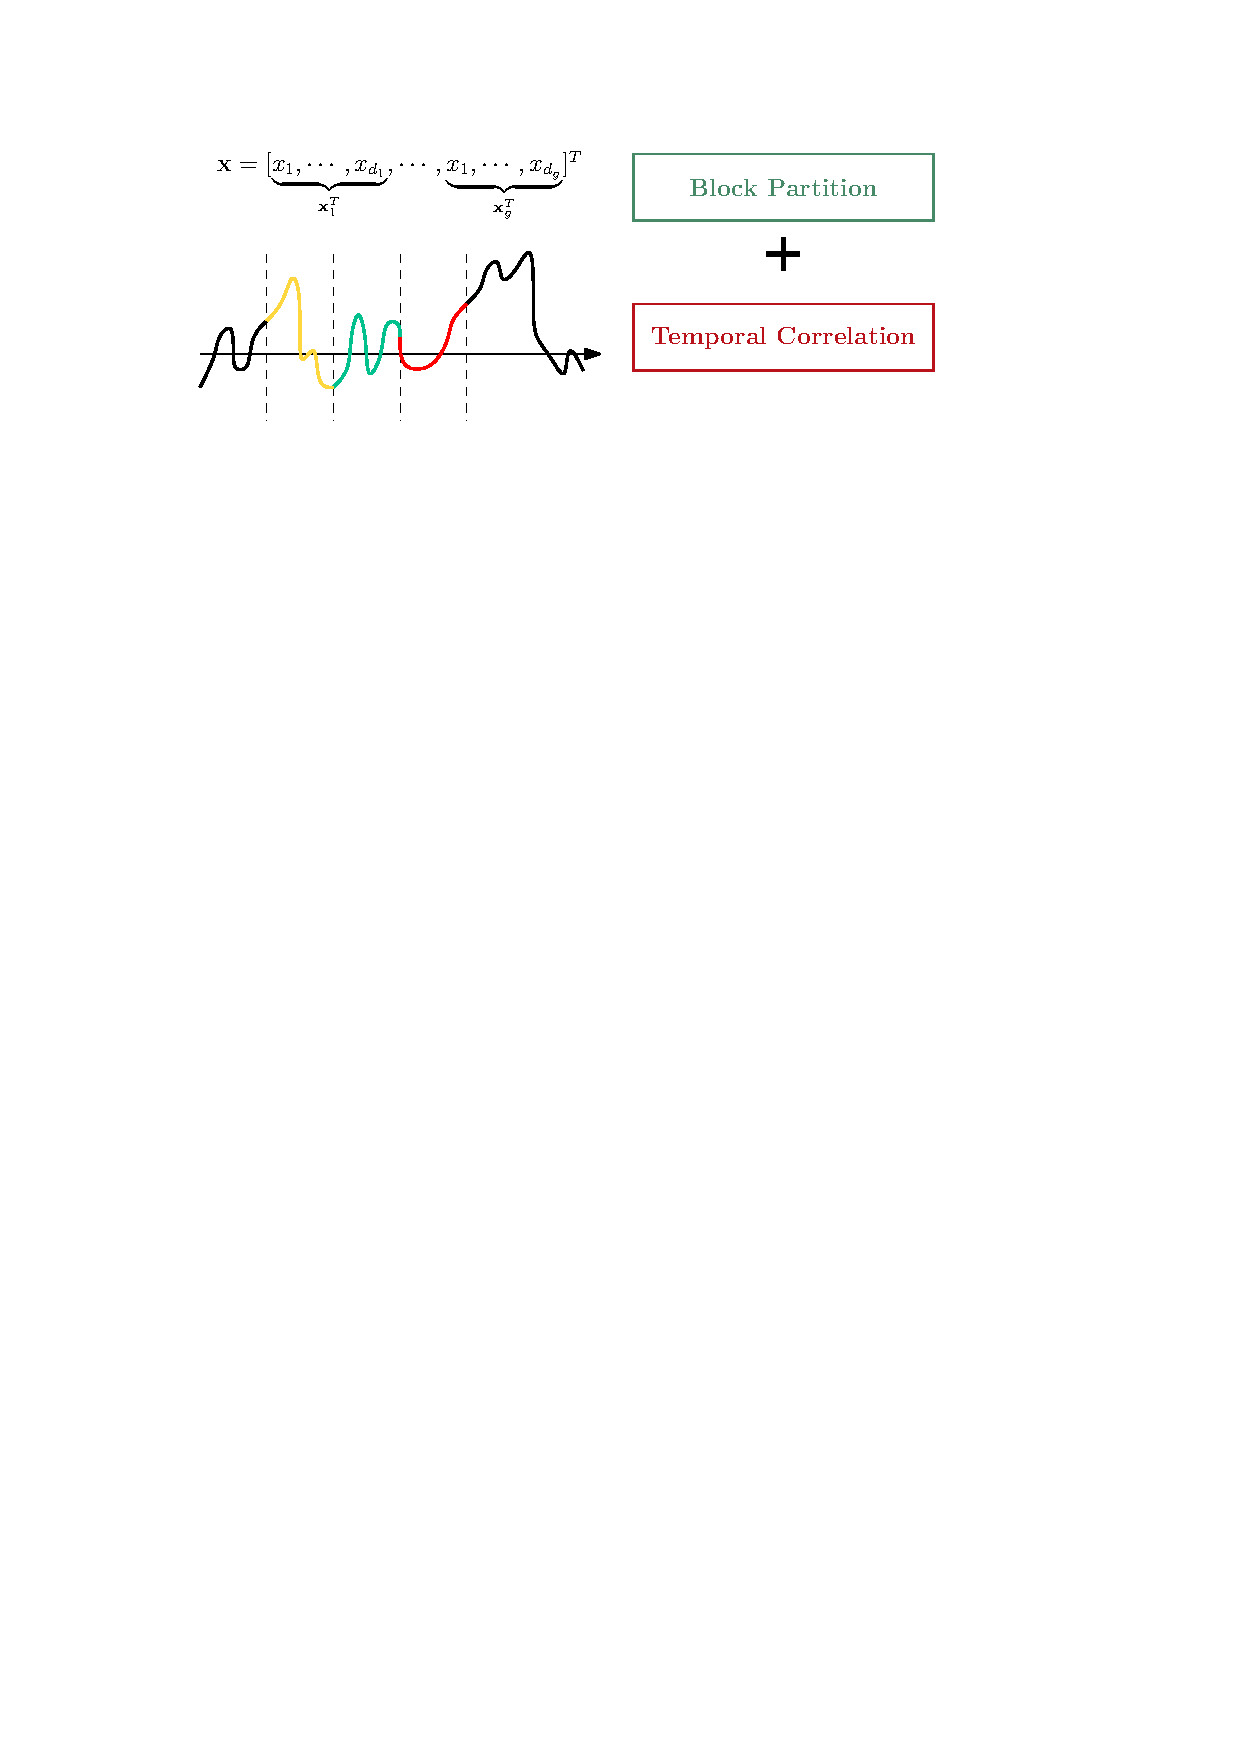
\includegraphics[width=.9\linewidth]{bsbl_block_plus_intra}}

    \begin{itemize}
        \item[1] Block Sparse Bayesian Learning (BSBL) exploits the \hl{temporal correlation} structures,
        \item[2] Abandoned \hl{block-sparsity} and assumed all blocks are \hl{non-zero}!
        \item[3] Successful and High-Fidelity.
    \end{itemize}
\end{frame}

%%------------------------------------------------------------------------%%
\begin{frame}{Spatio-Temporal : ST-SBL}

    \begin{minipage}{.3\linewidth}
        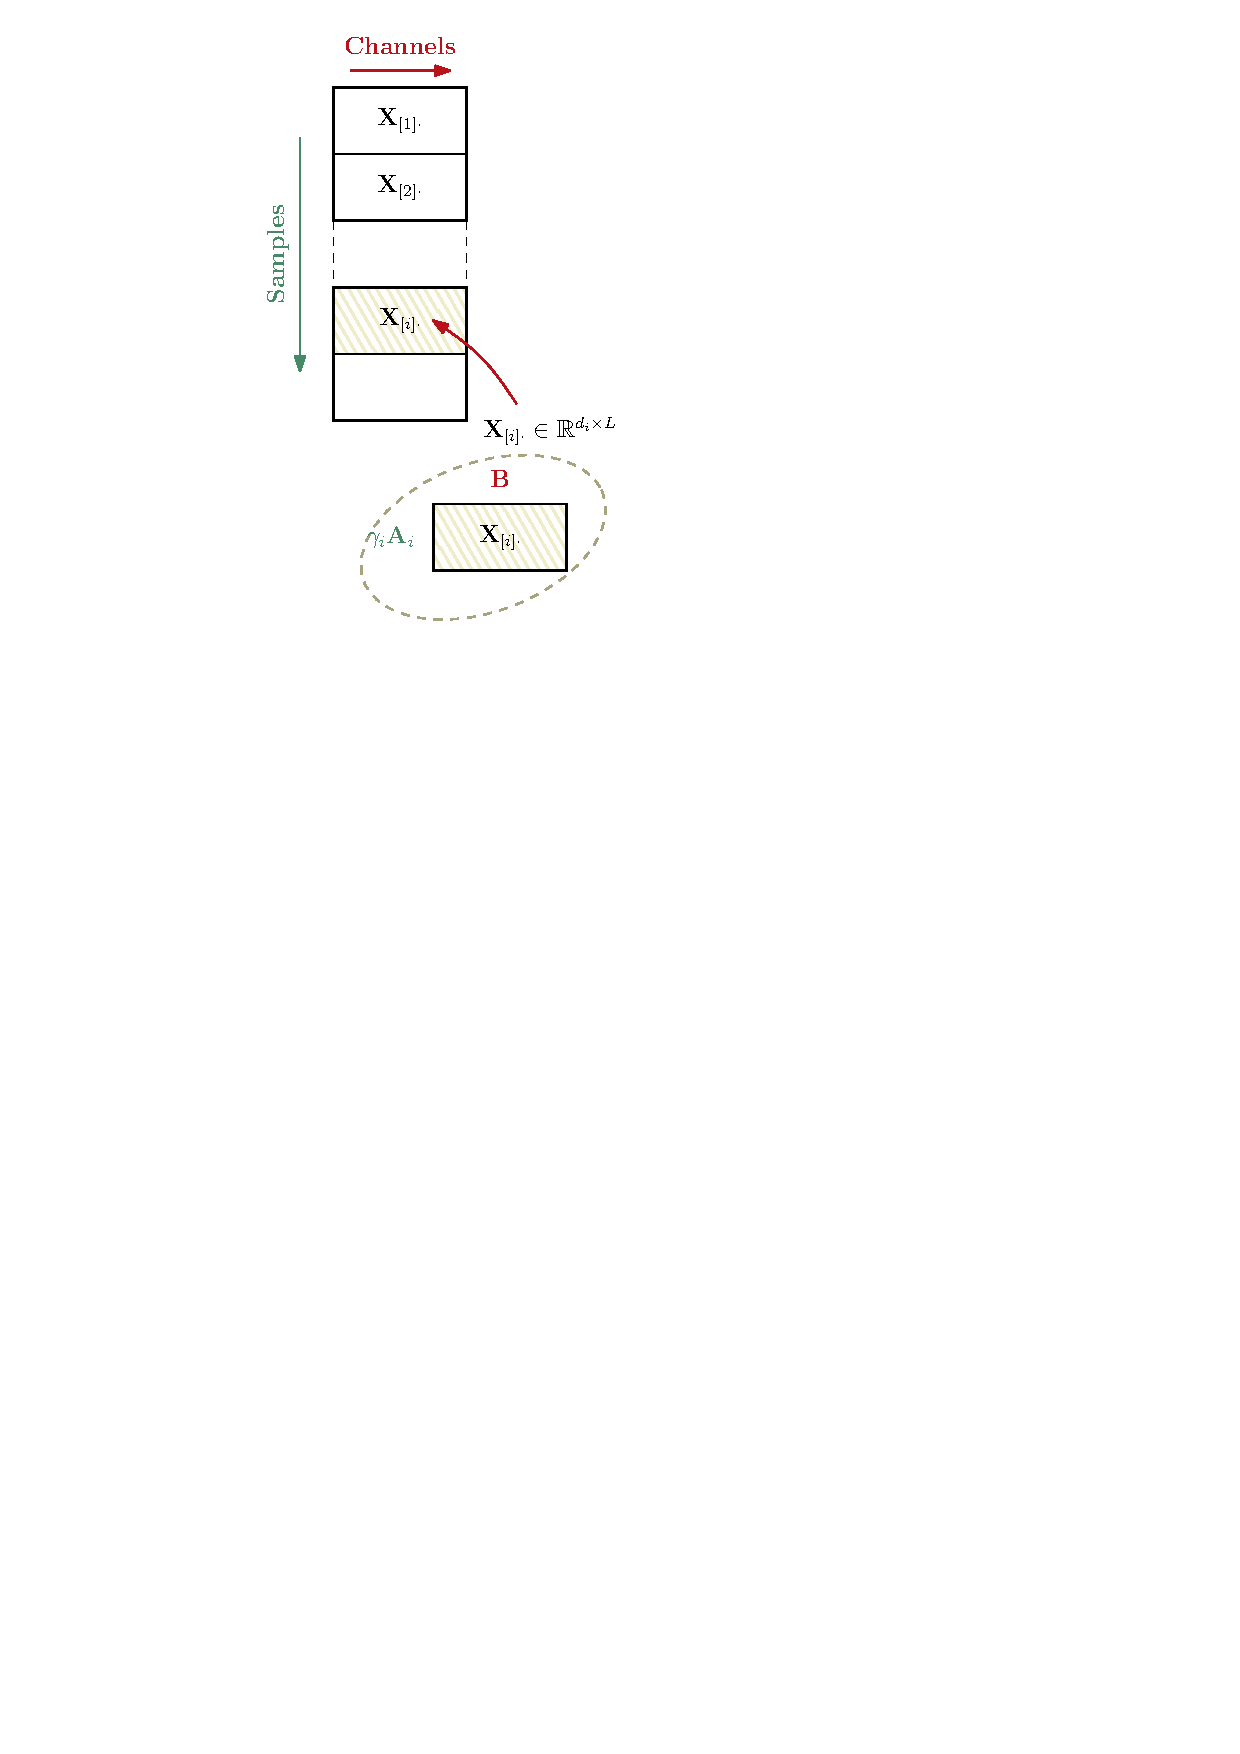
\includegraphics[width=\linewidth]{st-sbl_model}
    \end{minipage}
    \begin{minipage}{.68\linewidth}
        \begin{itemize}
            \item[1] $\ve{X}_{[i]\cdot}$ obeys parameterized Gaussian,
                \[
                    p(\mathrm{vec}(\ve{X}_{[i]\cdot});\gamma_i,\ve{B},\ve{A}_i) = \mathcal{N}(\ve{0},(\gamma_i\ve{A}_i)\otimes\ve{B})
                \]
                Blocks are mutually independent.
            \item[2] $\gamma_i$ determines whether the $i$th block is a zero block or not; $\ve{B}\in\mathbb{R}^{L\times L}$ is a p.s.d captures \hl{spatio correlation}; $\ve{A}_i\in\mathbb{R}^{d_i\times d_i}$ is an unknown p.s.d captures \hl{temporal correlation}.
            \item[3] The sensor noise $\ve{V}$ can be ignored : artifacts and noises are incorporate into $\ve{X}$.
        \end{itemize}
    \end{minipage}

\end{frame}

%%------------------------------------------------------------------------%%
\begin{frame}{ST-SBL : Alternating Optimize of $\gamma_i$, $\ve{A}_i$ and $\ve{B}$}
    
    \begin{minipage}{.39\linewidth}
        {\centering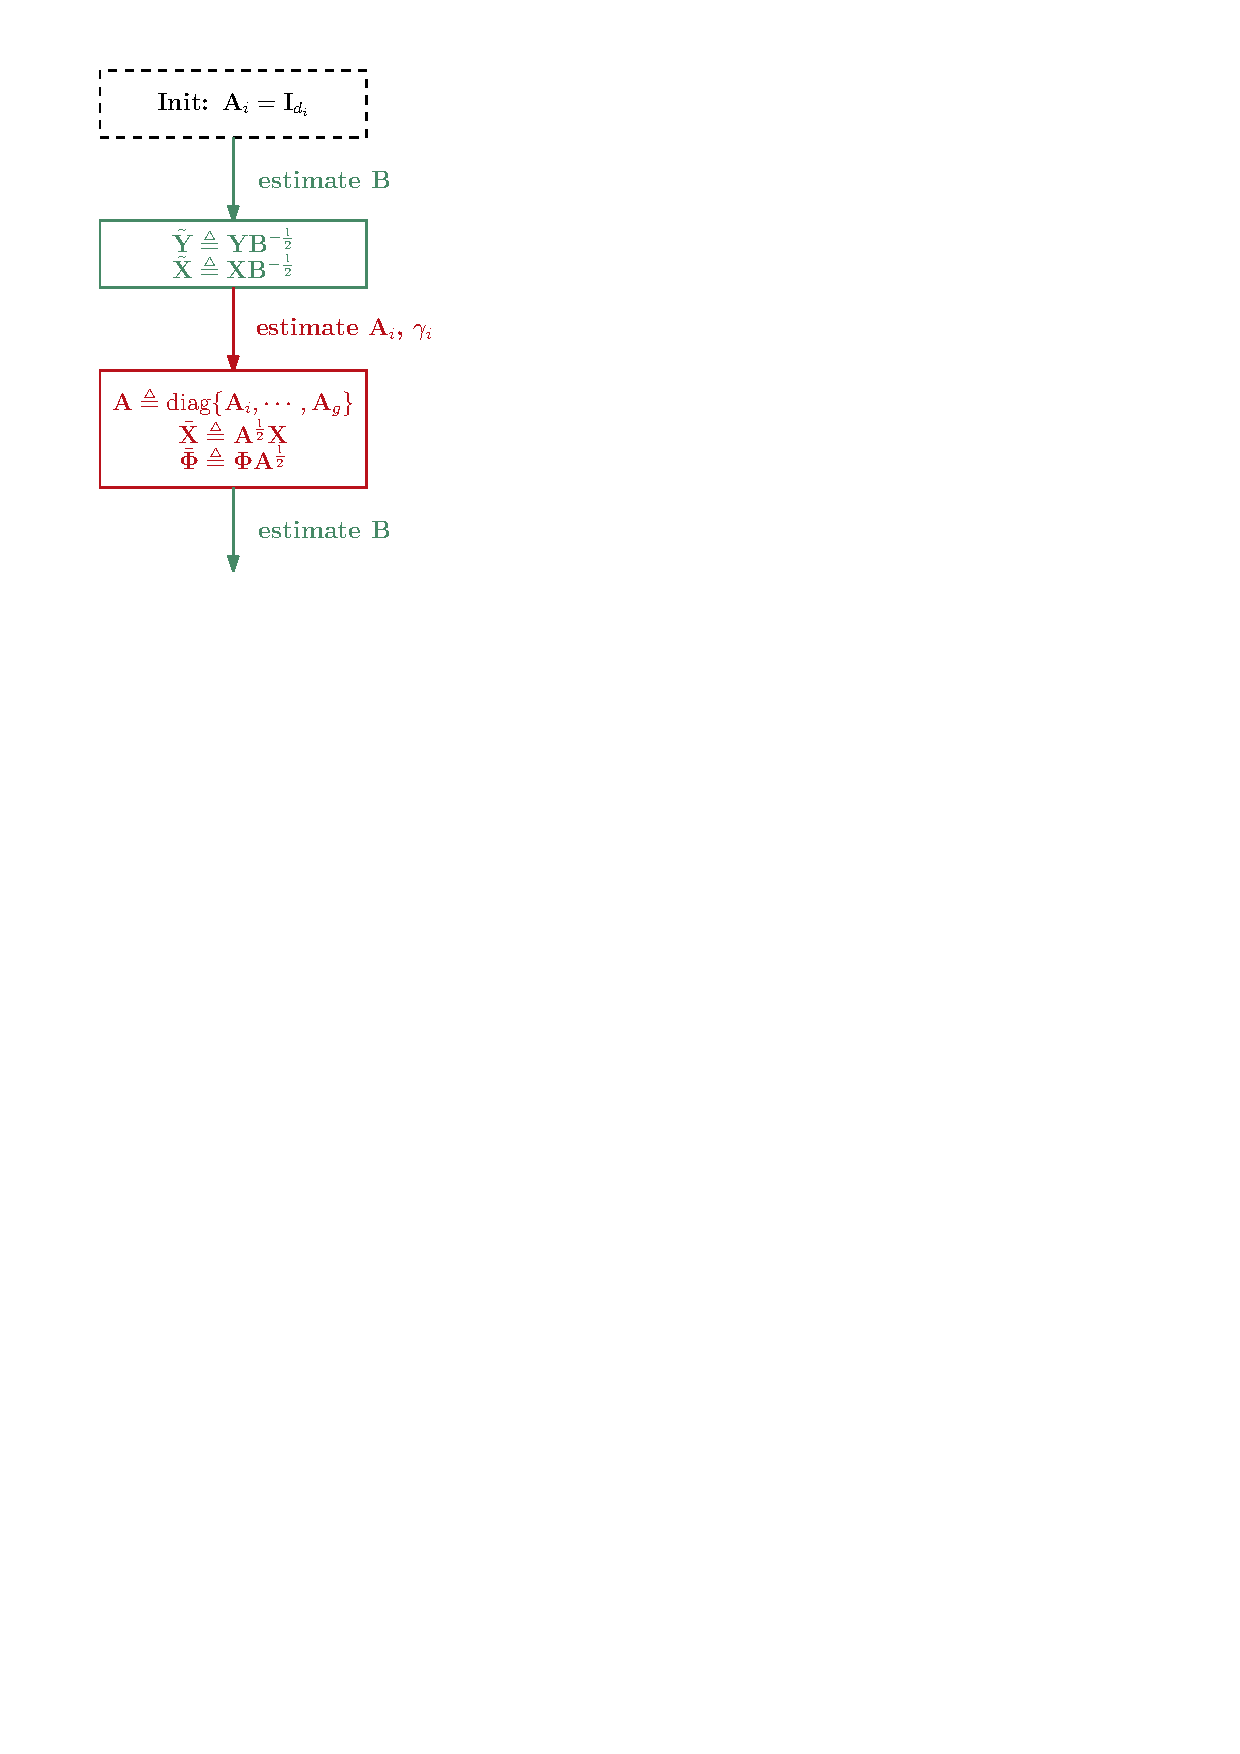
\includegraphics[width=\linewidth]{st-sbl_alternate}}
    \end{minipage}
    \begin{minipage}{.60\linewidth}
        \begin{itemize}
            \item[1] Estimating $\ve{B}$
                \[
                    \ve{B} = \sum_{i=1}^g \gamma_i \ve{X}_{[i]\cdot}^T\ve{A}_i^{-1}\ve{X}_{[i]\cdot}
                \]
            \item[2] Estimating $\gamma_i$, $\ve{A}_i$
                \[
                    \gamma_i = \frac{1}{Ld_i} \sum_{l=1}^L \mathrm{Tr}\left[\ve{A}_i^{-1}(\bm{\Sigma}_{[i]} + \bm{\mu}_{[i]l}^T\bm{\mu}_{[i]l})\right]
                \]
                \[
                    \ve{A}_i = \frac{1}{L} \sum_{l=1}^L \frac{\bm{\Sigma}_{[i]} + \bm{\mu}_{[i]l}^T\bm{\mu}_{[i]l}}{\gamma_i}
                \]
            \item[3] Updating $\ve{X}$
                \[
                    \ve{X} = \bm{\mu}\ve{B}^{\frac{1}{2}}
                \]
        \end{itemize}
    \end{minipage}

\end{frame}

%%------------------------------------------------------------------------%%
\begin{frame}{Applications : Drowsiness Monitoring Based on EEG}

    \magt{illustrate the background of driving drowsy and EEG collecting}
    {%
        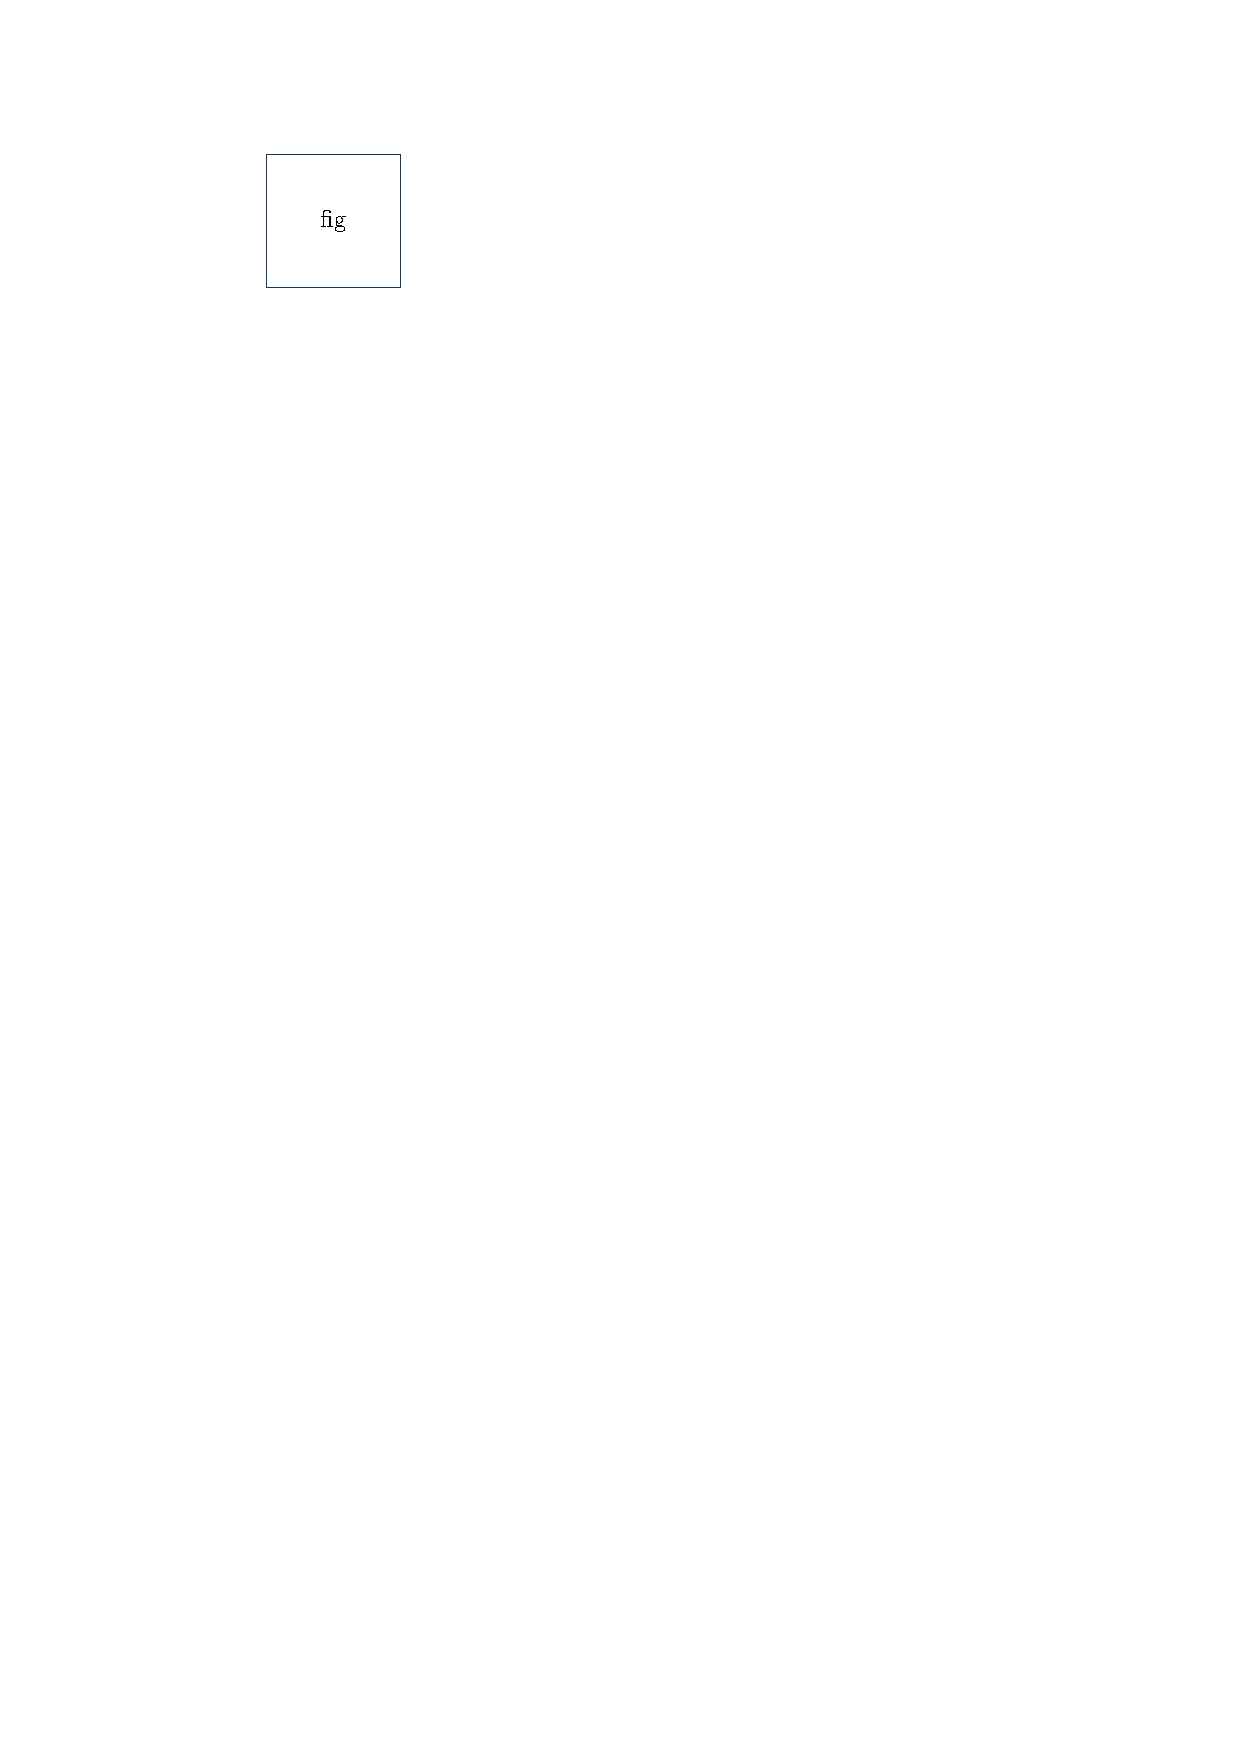
\includegraphics[width=.24\linewidth]{null}~
        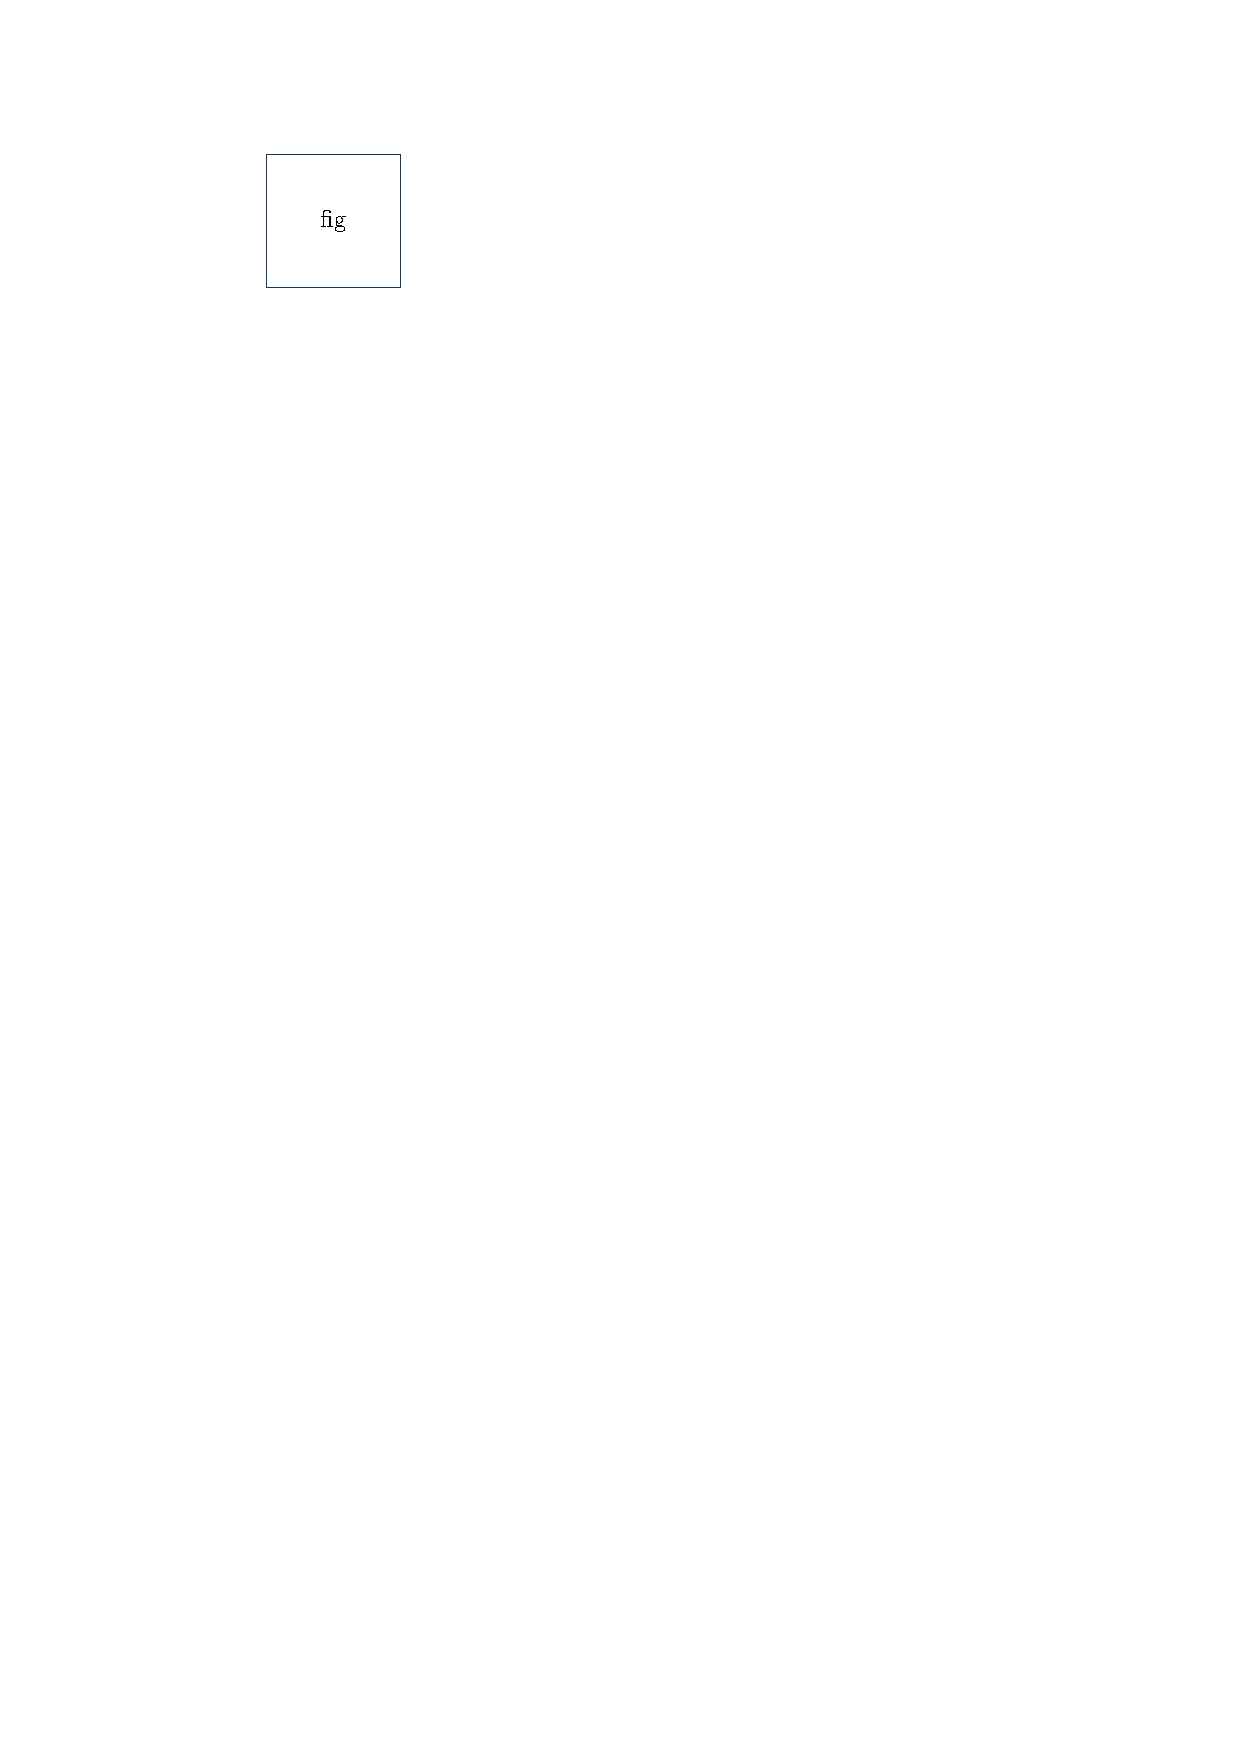
\includegraphics[width=.24\linewidth]{null}~
        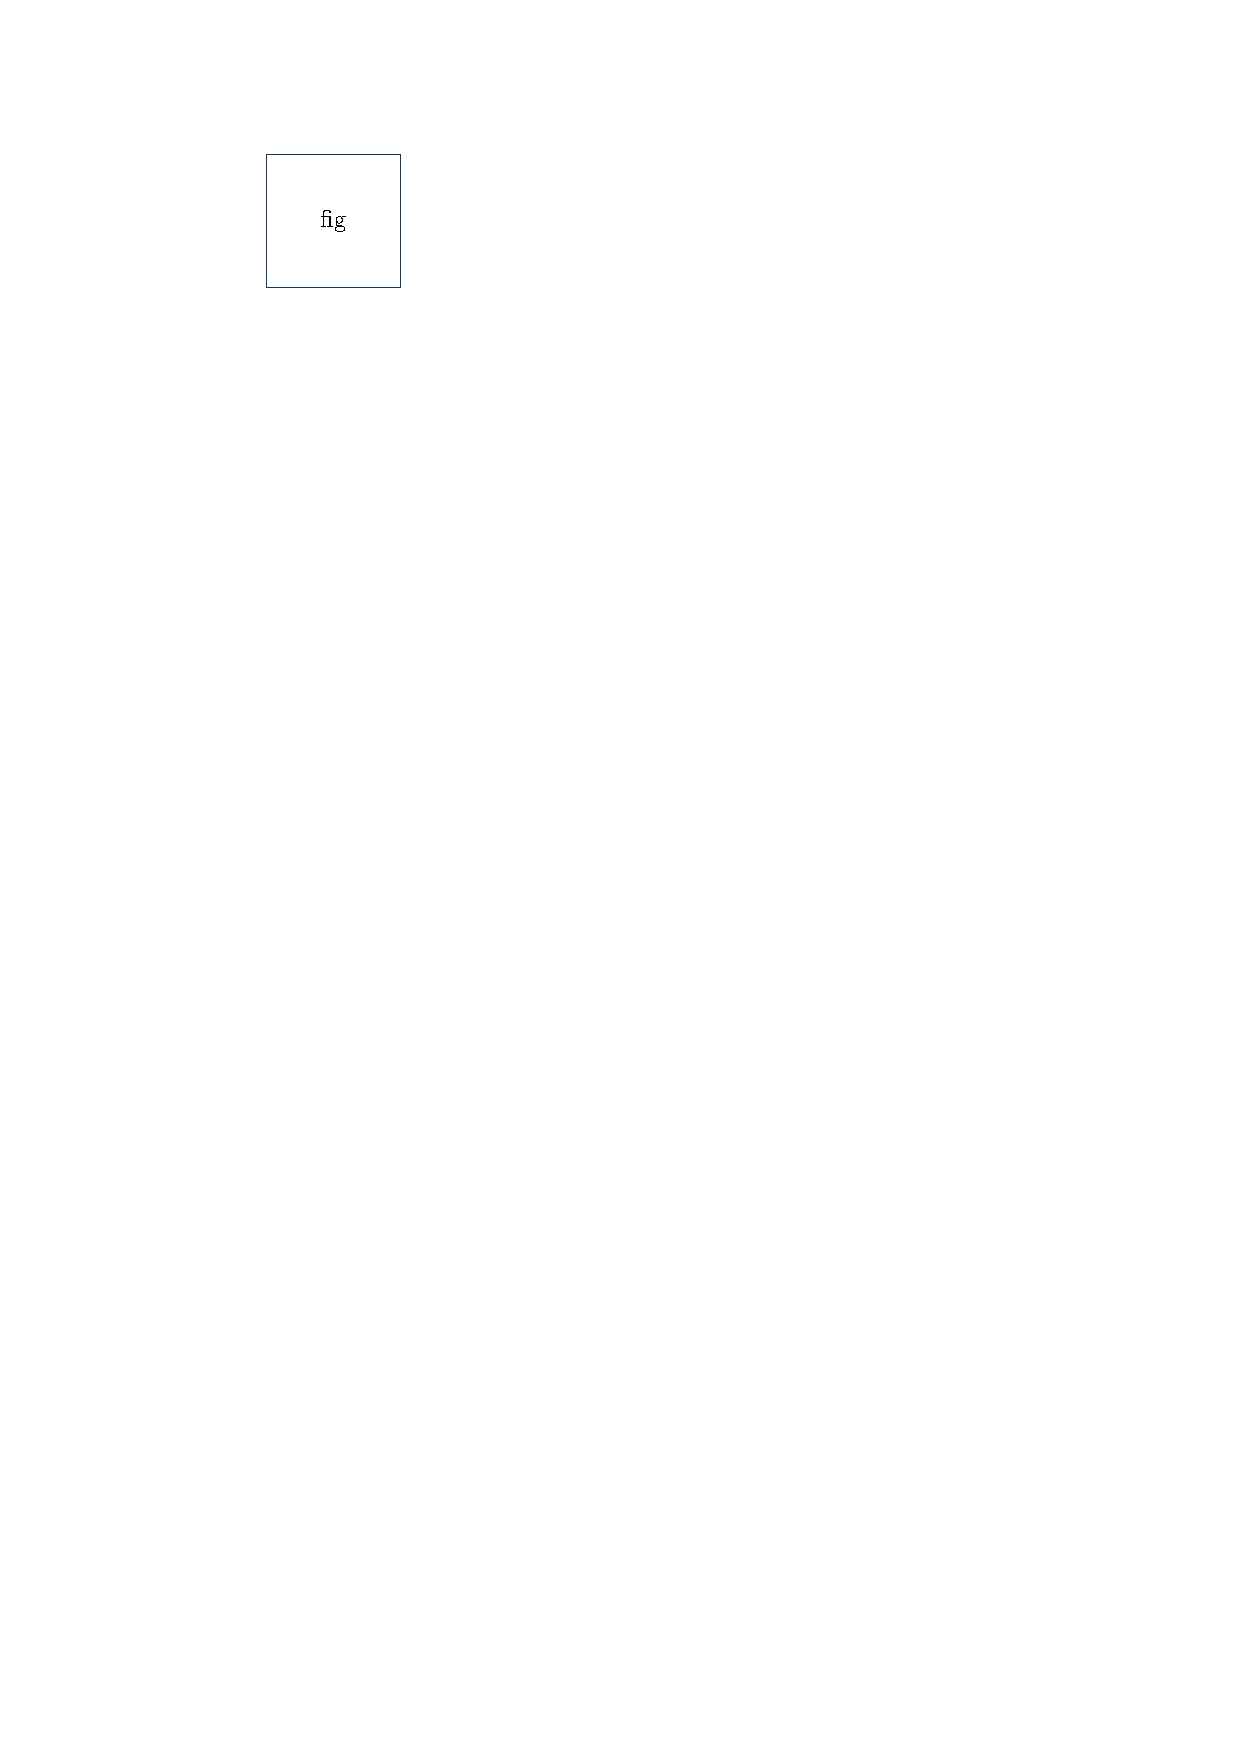
\includegraphics[width=.24\linewidth]{null}~
        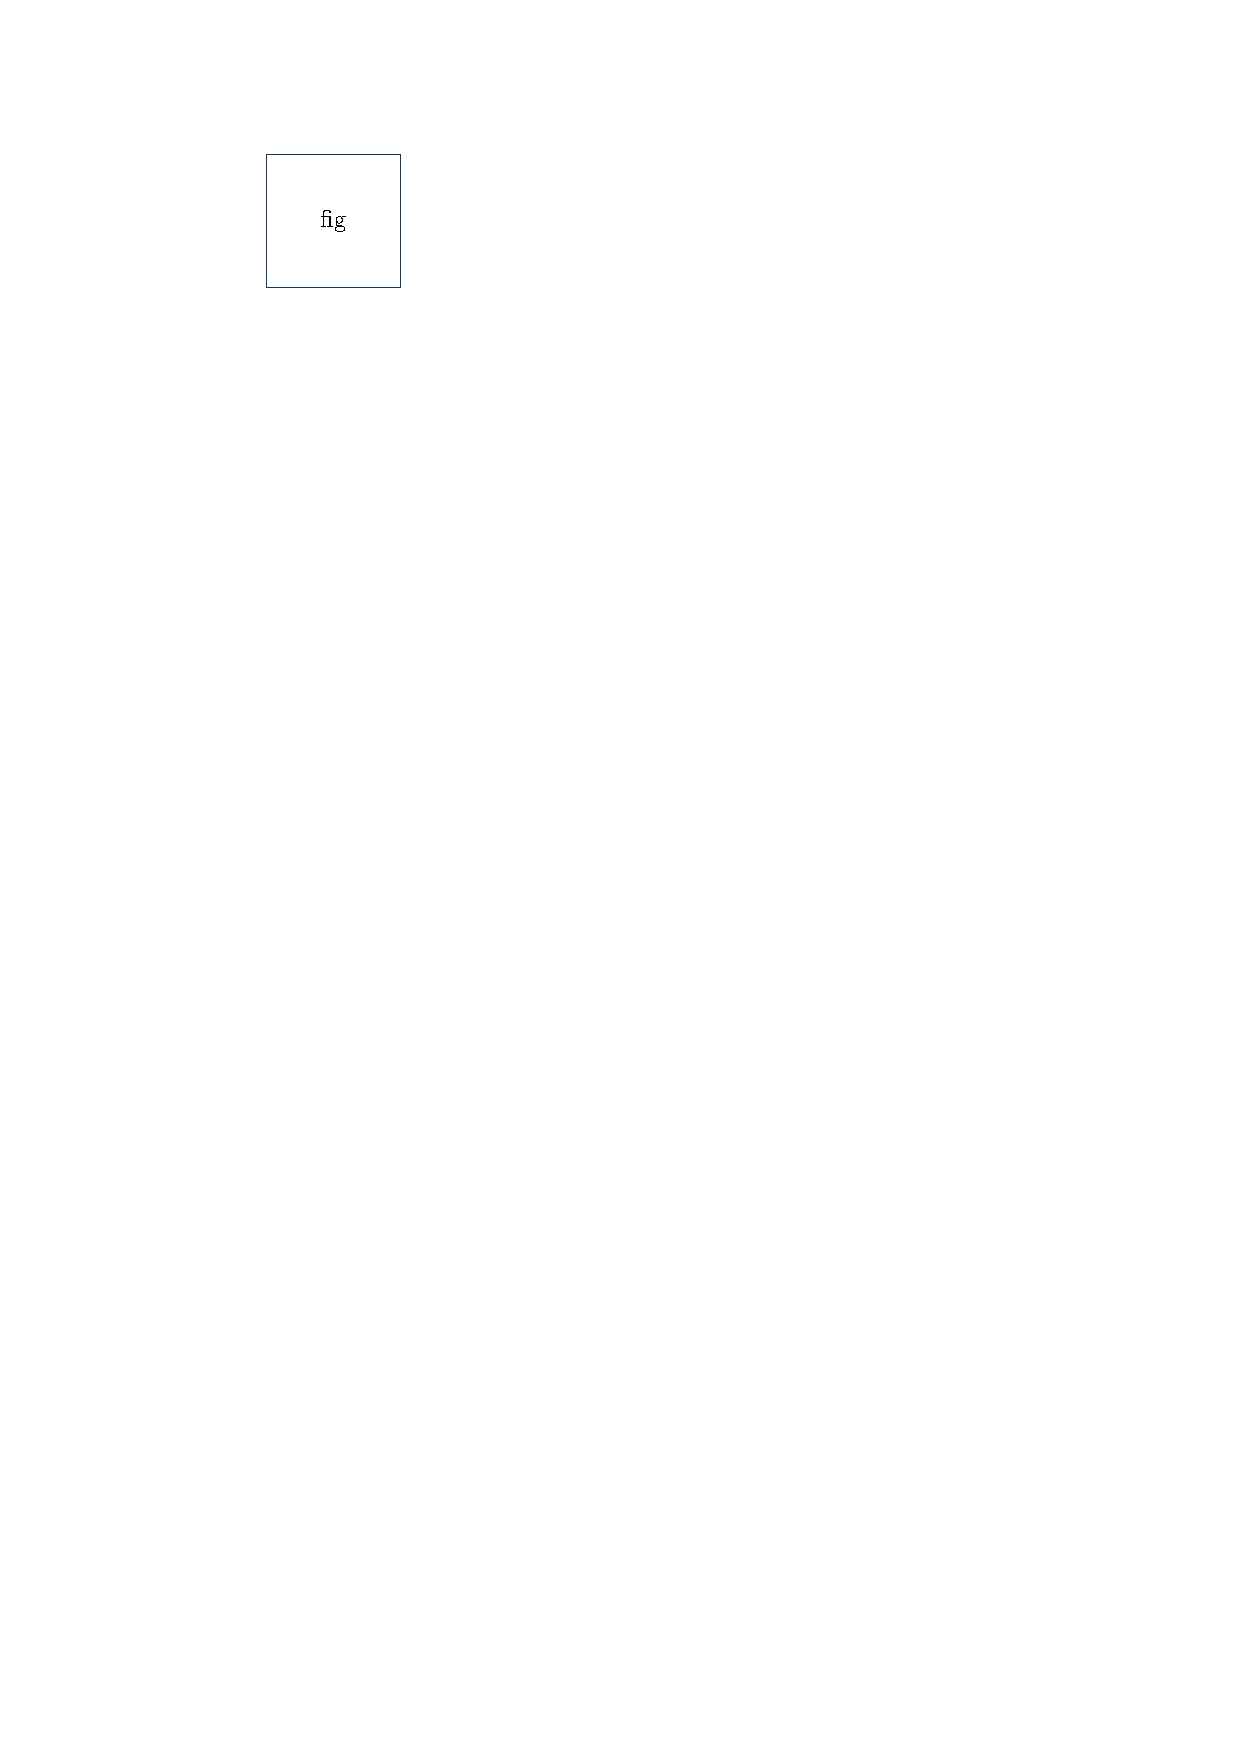
\includegraphics[width=.24\linewidth]{null}~
    }

    \begin{itemize}
        \item Compression Ratio
            \[
                \mathrm{CR} = \frac{M-N}{M}
            \]
        \item Task Driven Analysis (not MSE!)
            \centerline{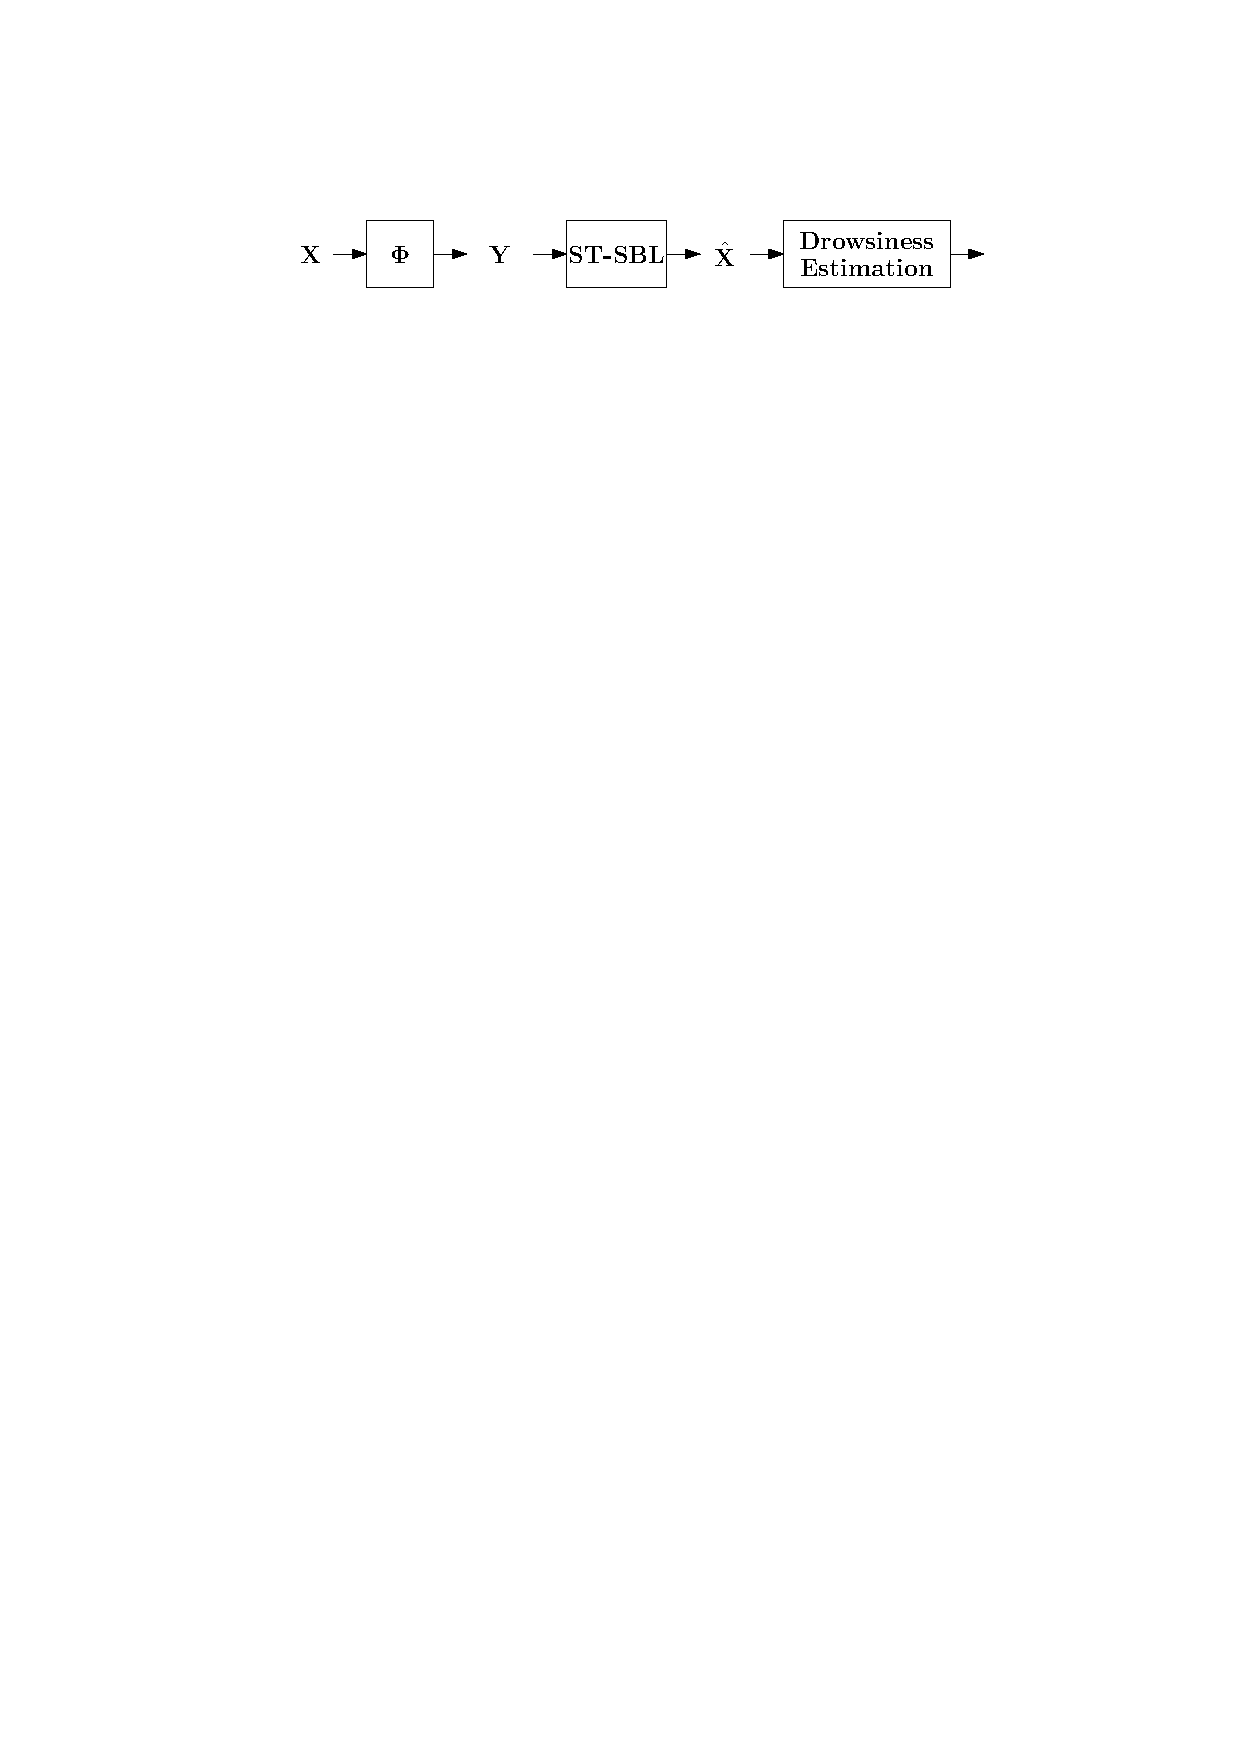
\includegraphics[width=.8\linewidth]{task_driven_drowsy}}
    \end{itemize}

\end{frame}


%%--------------------END--------------------%%
%\begin{frame}
%\begin{center}
%\vspace*{0.6cm}
%{\huge \emph{\textcolor{magenta}{That's all.}}}\\[5mm]
%{\huge \textsc{Any Questions?}}
%\vspace*{0.6cm}
%\begin{tabular}{ll}
%{\sc Author}: & Zhilin Zhang\\
%{\sc Title}: & Title\\
%{\sc Code}: & \magt{FTP}/public/lby \\
%{\sc Email}: & \href{mailto:liubenyuan@gmail.com}{\color{blue}liubenyuan@gmail.com} \\
%\end{tabular}
%\end{center}
%\end{frame}

\end{document}
% EOF
